%\RequirePackage[l2tabu, orthodox]{nag}
\documentclass[12pt]{beamer}
\graphicspath{{Imagenes/}{../Imagenes/}}
\usepackage[utf8]{inputenc}
\usepackage[spanish]{babel}
\usepackage[autostyle,spanish=mexican]{csquotes}
\usepackage{hyperref}
\hypersetup{
  colorlinks=true,
  linkcolor=blue,          % color of internal links (change box color with linkbordercolor)
  citecolor=green,        % color of links to bibliography
  filecolor=magenta,      % color of file links
  urlcolor=cyan,           % color of external links
  linkbordercolor={0 0 1}
}
\usepackage{amsmath}
\usepackage{amsthm}
\usepackage{multicol}
\usepackage{graphicx}
\usepackage{physics}
\usepackage{tabulary}
\usepackage{booktabs}
\usepackage[outdir=./]{epstopdf}
%\usepackage{epstopdf}
\usepackage{media9}
\usepackage{multimedia}
\usepackage[binary-units=true]{siunitx}
\usepackage{standalone}
\usepackage{longtable}
\usepackage{bigints}
\usepackage[font=footnotesize,textfont=it]{caption}
%\usepackage{enumitem}
\usepackage{tikz}
\usetikzlibrary{mindmap}
\usepackage[siunitx]{circuitikz}
\usetikzlibrary{arrows, patterns, shapes, decorations.markings, decorations.pathmorphing}
\usetikzlibrary{matrix,positioning}
\tikzstyle{every picture}+=[remember picture,baseline]
\usepackage{color}
\usepackage{alltt}
\usepackage{verbatim}
\usepackage{colortbl}
\usepackage{fancyvrb}
\usepackage[os=win]{menukeys}
\usepackage{pifont}
\usepackage[sfdefault]{roboto}  %% Option 'sfdefault' only if the base font of the document is to be sans serif
%\usepackage[T1]{fontenc}
\setcounter{secnumdepth}{3}
\setcounter{tocdepth}{3}
\DeclareGraphicsExtensions{.pdf,.png,.jpg}
\renewcommand {\arraystretch}{1.5}
\definecolor{ao}{rgb}{0.0, 0.5, 0.0}
\definecolor{bisque}{rgb}{1.0, 0.89, 0.77}
\definecolor{amber}{rgb}{1.0, 0.75, 0.0}
\definecolor{armygreen}{rgb}{0.29, 0.33, 0.13}
\definecolor{alizarin}{rgb}{0.82, 0.1, 0.26}
\definecolor{cadetblue}{rgb}{0.37, 0.62, 0.63}
\newcommand*{\TitleParbox}[1]{\parbox[c]{6cm}{\raggedright #1}}%
\newcommand{\python}{\texttt{python}}
\newcommand{\textoazul}[1]{\textcolor{blue}{#1}}
\newcommand{\azulfuerte}[1]{\textcolor{blue}{\textbf{#1}}}
\newcommand{\funcionazul}[1]{\textcolor{blue}{\textbf{\texttt{#1}}}}
%\normalfont
\usepackage{ccfonts}% http://ctan.org/pkg/{ccfonts}
\usepackage[T1]{fontenc}% http://ctan.or/pkg/fontenc
\renewcommand{\rmdefault}{cmr}% cmr = Computer Modern Roman
\usefonttheme[onlymath]{serif}
\linespread{1.3}
\newcounter{saveenumi}
\newcommand{\seti}{\setcounter{saveenumi}{\value{enumi}}}
\newcommand{\conti}{\setcounter{enumi}{\value{saveenumi}}}
\newcommand{\tikzmark}[1]{\tikz[remember picture] \node[coordinate] (#1) {#1};}

\usepackage{scalerel}[2016-12-29]
\def\stretchint#1{\vcenter{\hbox{\stretchto[440]{\displaystyle\int}{#1}}}}
\def\scaleint#1{\vcenter{\hbox{\scaleto[3ex]{\displaystyle\int}{#1}}}}
\def\bs{\mkern-12mu}

\newtheorem{teo}{}[section]
\usepackage{blkarray}

%reduce el tamaño de letra de la etiqueta equations
\makeatletter
\def\maketag@@@#1{\hbox{\m@th\normalfont\small#1}}
\makeatother

%se usa para la x en itemize
\newcommand{\xmark}{\text{\ding{55}}}

%\AtBeginDocument{\setlength{\tymin}{1em}}


\definecolor{myblue}{rgb}{.8, .8, 1}

\usepackage{amsmath}
\usepackage{empheq}

\newlength\mytemplen
\newsavebox\mytempbox

\makeatletter
\newcommand\mybluebox{%
    \@ifnextchar[%]
       {\@mybluebox}%
       {\@mybluebox[0pt]}}

\def\@mybluebox[#1]{%
    \@ifnextchar[%]
       {\@@mybluebox[#1]}%
       {\@@mybluebox[#1][0pt]}}

\def\@@mybluebox[#1][#2]#3{
    \sbox\mytempbox{#3}%
    \mytemplen\ht\mytempbox
    \advance\mytemplen #1\relax
    \ht\mytempbox\mytemplen
    \mytemplen\dp\mytempbox
    \advance\mytemplen #2\relax
    \dp\mytempbox\mytemplen
    \colorbox{myblue}{\hspace{1em}\usebox{\mytempbox}\hspace{1em}}}

\makeatother



%Se usa la plantilla Warsaw modificada con whale
\mode<presentation>
{
  \usetheme{Warsaw}
  \setbeamertemplate{headline}{}
  %\useoutertheme{infolines}
  \usecolortheme{whale}
  \setbeamercovered{invisible}
  

 \setbeamertemplate{section in toc}[sections numbered]
 \setbeamertemplate{subsection in toc}[subsections numbered]
 \setbeamertemplate{subsection in toc}{\leavevmode\leftskip=3.2em\rlap{\hskip-2em\inserttocsectionnumber.\inserttocsubsectionnumber}\inserttocsubsection\par}
% \setbeamercolor{section in toc}{fg=blue}
 \setbeamercolor{subsection in toc}{fg=blue}
 \setbeamerfont{subsection in toc}{size=\small}


\setbeamertemplate{navigation symbols}{}
\setbeamertemplate{caption}[numbered]
% \setbeamercolor{frametitle}{fg=yellow,bg=blue!70!white}
\setbeamercolor{section in head/foot}{bg=black, fg=white}
%\setbeamercolor{subsection in head/foot}{bg=gray!30,fg=black}
%\setbeamercolor{author in head/foot}{fg=yellow}
%\setbeamercolor{date in head/foot}{fg=blue}

%\mode<presentation>
%{
%  \usetheme{Warsaw}
%  \setbeamertemplate{headline}{}
%  %\useoutertheme{infolines}
%  \useoutertheme{default}
%  \setbeamercovered{invisible}
%  % or whatever (possibly just delete it)
%}
}


\usepackage{courier}
\usepackage{listingsutf8}
\usepackage{listings}
\usepackage{xcolor}
\usepackage{textcomp}
\usepackage{color}
\definecolor{deepblue}{rgb}{0,0,0.5}
\definecolor{brown}{rgb}{0.59, 0.29, 0.0}
\definecolor{OliveGreen}{rgb}{0,0.25,0}
% \usepackage{minted}

\DeclareCaptionFont{white}{\color{white}}
\DeclareCaptionFormat{listing}{\colorbox{gray}{\parbox{0.98\textwidth}{#1#2#3}}}
\captionsetup[lstlisting]{format=listing,labelfont=white,textfont=white}
\renewcommand{\lstlistingname}{Código}


\definecolor{Code}{rgb}{0,0,0}
\definecolor{Keywords}{rgb}{255,0,0}
\definecolor{Strings}{rgb}{255,0,255}
\definecolor{Comments}{rgb}{0,0,255}
\definecolor{Numbers}{rgb}{255,128,0}

\makeatletter

\newif\iffirstchar\firstchartrue
\newif\ifstartedbyadigit
\newif\ifprecededbyequalsign

\newcommand\processletter
{%
  \ifnum\lst@mode=\lst@Pmode%
    \iffirstchar%
        \global\startedbyadigitfalse%
      \fi
      \global\firstcharfalse%
    \fi
}

\newcommand\processdigit
{%
  \ifnum\lst@mode=\lst@Pmode%
      \iffirstchar%
        \global\startedbyadigittrue%
      \fi
      \global\firstcharfalse%
  \fi
}

\lst@AddToHook{OutputOther}%
{%
  \lst@IfLastOtherOneOf{=}
    {\global\precededbyequalsigntrue}
    {}%
}

\lst@AddToHook{Output}%
{%
  \ifprecededbyequalsign%
      \ifstartedbyadigit%
        \def\lst@thestyle{\color{orange}}%
      \fi
    \fi
  \global\firstchartrue%
  \global\startedbyadigitfalse%
  \global\precededbyequalsignfalse%
}

\lstset{ 
language=Python,                % choose the language of the code
basicstyle=\footnotesize\ttfamily,       % the size of the fonts that are used for the code
numbers=left,                   % where to put the line-numbers
numberstyle=\scriptsize,      % the size of the fonts that are used for the line-numbers
stepnumber=1,                   % the step between two line-numbers. If it is 1 each line will be numbered
numbersep=5pt,                  % how far the line-numbers are from the code
backgroundcolor=\color{white},  % choose the background color. You must add \usepackage{color}
showspaces=false,               % show spaces adding particular underscores
showstringspaces=false,         % underline spaces within strings
showtabs=false,                 % show tabs within strings adding particular underscores
frame=single,   		% adds a frame around the code
tabsize=2,  		% sets default tabsize to 2 spaces
captionpos=t,   		% sets the caption-position to bottom
breaklines=true,    	% sets automatic line breaking
breakatwhitespace=false,    % sets if automatic breaks should only happen at whitespace
escapeinside={| |},  % if you want to add a comment within your code
stringstyle =\color{OliveGreen},
otherkeywords={as, np.array, np.concatenate, np.linspace, linspace, interpolate.interp1d, kind, plt.plot, .copy, np.arange, np.cos, np.pi, lw, ls, label, splrep, splev, plt.legend, loc, plt.title, plt.ylim, plt.show, sign, math.ceil, math.log, np.sqrt, np.exp, np.zeros, plt.xlabel, plt.ylabel, plt.xlim, np.identity, random, np.dot, np.outer, np.diagonal },             % Add keywords here
keywordstyle = \color{blue},
commentstyle = \color{darkcerulean},
identifierstyle = \color{black},
literate=%
         {á}{{\'a}}1
         {é}{{\'e}}1
         {í}{{\'i}}1
         {ó}{{\'o}}1
         {ú}{{\'u}}1
%
%keywordstyle=\ttb\color{deepblue}
%fancyvrb = true,
}

\lstdefinestyle{FormattedNumber}{%
    literate={0}{{\textcolor{red}{0}}}{1}%
             {1}{{\textcolor{red}{1}}}{1}%
             {2}{{\textcolor{red}{2}}}{1}%
             {3}{{\textcolor{red}{3}}}{1}%
             {4}{{\textcolor{red}{4}}}{1}%
             {5}{{\textcolor{red}{5}}}{1}%
             {6}{{\textcolor{red}{6}}}{1}%
             {7}{{\textcolor{red}{7}}}{1}%
             {8}{{\textcolor{red}{8}}}{1}%
             {9}{{\textcolor{red}{9}}}{1}%
             {.0}{{\textcolor{red}{.0}}}{2}% Following is to ensure that only periods
             {.1}{{\textcolor{red}{.1}}}{2}% followed by a digit are changed.
             {.2}{{\textcolor{red}{.2}}}{2}%
             {.3}{{\textcolor{red}{.3}}}{2}%
             {.4}{{\textcolor{red}{.4}}}{2}%
             {.5}{{\textcolor{red}{.5}}}{2}%
             {.6}{{\textcolor{red}{.6}}}{2}%
             {.7}{{\textcolor{red}{.7}}}{2}%
             {.8}{{\textcolor{red}{.8}}}{2}%
             {.9}{{\textcolor{red}{.9}}}{2}%
             {\ }{{ }}{1}% handle the space
         ,%
          %mathescape=true
          escapeinside={__}
          }



\makeatletter

% \setbeamercolor{subsection in foot}{bg=blue!30!yellow, fg=red}
%\setbeamercolor{footlinecolor}{bg=black,fg=white}
\setbeamertemplate{footline}
{
  \leavevmode%
  \hbox{%
  \begin{beamercolorbox}[wd=.333333\paperwidth,ht=2.25ex,dp=1ex,center]{section in footline}%
    \usebeamerfont{section in foot} \insertsection
  \end{beamercolorbox}}%
  \begin{beamercolorbox}[wd=.333333\paperwidth,ht=2.25ex,dp=1ex,center]{subsection in foot}%
    \usebeamerfont{subsection in foot}  \insertsubsection
  \end{beamercolorbox}%
  \begin{beamercolorbox}[wd=.333333\paperwidth,ht=2.25ex,dp=1ex,right]{date in head/foot}%
    \usebeamerfont{date in head/foot} \insertshortdate{} \hspace*{2em}
    \insertframenumber{} / \inserttotalframenumber \hspace*{2ex} 
  \end{beamercolorbox}}%
  \vskip0pt%
\makeatother
\normalfont
\usepackage{ccfonts}% http://ctan.org/pkg/{ccfonts}
\usepackage[T1]{fontenc}% http://ctan.or/pkg/fontenc
\renewcommand{\rmdefault}{cmr}% cmr = Computer Modern Roman
\linespread{1.3}
\title{EDO con condiciones de frontera}
\subtitle{Curso de Física Computacional}
\author{M. en C. Gustavo Contreras Mayén}
\date{\today}
\institute{Facultad de Ciencias - UNAM}
\titlegraphic{
\includegraphics[width=1.75cm]{Imagenes/escudo-facultad-ciencias.jpg}\hspace*{4.75cm}~%
   
\includegraphics[width=1.75cm]{Imagenes/escudo-unam.jpg}
}
\begin{document}
\maketitle
\fontsize{14}{14}\selectfont
\spanishdecimal{.}
\section*{Contenido}
\frame{\tableofcontents[currentsection, hideallsubsections]}
\section{Método de diferencias finitas}
\frame{\tableofcontents[currentsection, hideothersubsections]}
\subsection{Definición}
%Referencia Titu Cap. 12
\begin{frame}
\frametitle{ED con condiciones de frontera}
Entre los métodos numéricos para resolver problemas con CDF, se sabe que los métodos de diferencias finitas tienen las mejores propiedades de estabilidad.
\\
\bigskip
Es cierto, sin embargo, que la estabilidad mejorada se produce, en general, a expensas de un mayor esfuerzo computacional para una precisión comparable.
\end{frame}
\begin{frame}
\frametitle{Método de diferencias finitas}
Esencialmente, los métodos de diferencias finitas implican aproximar las derivadas en la EDO y las CDF, mediante esquemas de diferencias finitas definidos en un conjunto discreto de puntos de una malla.
\end{frame}
\begin{frame}
\frametitle{Método de diferencias finitas}
En cualquier caso, se supone que los esquemas de discretización particulares utilizados aseguran un orden homogéneo de los errores de truncamiento.
\\
\bigskip
El sistema resultante de ecuaciones algebraicas puede resolverse mediante un método, o en el caso ideal, mediante un método adaptado a la forma particular del sistema.
\end{frame}
\begin{frame}
\frametitle{Forma general de la EDO con CDF}
Consideremos el problema lineal con CDF
\begin{equation}
y^{\prime \prime} =  p(x) \: y^{\prime} +  q(x) \: y + r(x)
\label{eq:ecuacion_12_93} 
\end{equation}
y con las condiciones
\begin{align}
\begin{aligned}
\alpha_{1} \: y(x_{a}) + \beta_{1} \: y^{\prime}(x_{a}) &= 1 \\
\alpha_{2} \: y(x_{b}) + \beta_{2} \: y^{\prime}(x_{b}) &= 1
\end{aligned}
\label{eq:ecuacion_12_94}
\end{align}
donde suponemos que $p(x)$, $q(x)$ y $r(x)$ son funciones continuas en el intervalo $[x_{a}, x_{b}]$
\end{frame}
\begin{frame}
\frametitle{Condiciones de frontera}
Las condiciones de frontera están definidas por los cuatro coeficientes $\alpha_{1}$, $\beta_{1}$, $\alpha_{2}$ y $\beta_{2}$.
\\
\bigskip
Por lo que debe aplicarse la condición natural adicional: que ambos coeficientes $\alpha$ y $\beta$ para una frontera dada, no pueden ser iguales a 0, es decir:
\[ \vert \alpha_{i} \vert + \vert \beta_{i} \vert \neq 0, \hspace{0.5cm} i = 1, 2 \]
\end{frame}
\begin{frame}
\frametitle{Tipos de CDF}
En particular:
\setbeamercolor{item projected}{bg=blue!70!black,fg=white}
\setbeamertemplate{enumerate items}[circle]
\begin{enumerate}[<+->]
\item Para $\beta_{i} = 0$, se tiene una \emph{condición de frontera de tipo Dirichlet}, la cual define el valor de la solución en la frontera.
\item Para $\alpha_{i} = 0$, se tiene una \emph{condición de frontera de tipo Neumann}, que fija la solución de la derivada en la frontera.
\end{enumerate}
\pause
Los tipos de condición son distintos en las dos fronteras, dependiendo del problema en cuestión.
\end{frame}
\begin{frame}
\frametitle{Definición de la malla}
Consideremos una partición en el dominio $[x_{a}, x_{b}]$, definido por una malla de puntos equidistantes:
\begin{equation}
x_{m} = x_{a} + (m - 1) \: h, \hspace{1cm} m = 1, 2, \ldots, M
\label{eq:ecuacion_12_95}
\end{equation}
con una separación de igual tamaño
\begin{equation}
h = \dfrac{x_{b} - x_{a}}{M - 1}
\end{equation}
\label{eq:ecuacion_12_96}
\end{frame}
\subsection{Diferenciación}
\begin{frame}
\frametitle{Diferenciación}
Haciendo la notación $y_{m} \equiv y(x_{m})$, recurrimos a una aproximación discreta de la primera y segunda derivada: $y^{\prime}_{m}$ y $y^{\prime \prime}_{m}$, a partir del desarrollo de la serie de Taylor en $x_{m + 1} = x_{m} + h$ y $x_{m - 1} = x_{m} - h$:
\end{frame}
\begin{frame}
\frametitle{Diferenciación}
\begin{align}
y_{m + 1}&= y_{m} + h \: y^{\prime}_{m} + \dfrac{h^{2}}{2!} \: y^{\prime \prime}_{m} + \dfrac{h^{3}}{3!} \: y^{3}_{m} + O(h^{4}) \label{eq:ecuacion_12_97} \\
\nonumber \\
y_{m - 1} &= y_{m} - h \: y^{\prime}_{m} + \dfrac{h^{2}}{2!} \: y^{\prime \prime}_{m} - \dfrac{h^{3}}{3!} \: y^{3}_{m} + O(h^{4}) \label{eq:ecuacion_12_98}
\end{align}
\end{frame}
\begin{frame}
\frametitle{Primera derivada}
Para la primera derivada $y^{\prime}_{m}$, podemos obtenerla mediante aproximaciones directas, al truncar hasta  $(h^{2}/2) \: y^{\prime \prime}$ y cancelar todos los términos de orden mayor:
\begin{align}
\begin{aligned}
y^{\prime}_{m} &= \dfrac{y_{m} - y_{m - 1}}{h} + O(h) \\
y^{\prime}_{m} &= \dfrac{y_{m + 1} - y_{m}}{h} + O(h)
\end{aligned}
\label{eq:ecuacion_12_99}
\end{align}
que al dividirse entre $h$, queda solamente $O(h)$.
\end{frame}
\begin{frame}
\frametitle{Fórmulas de diferencias}
La primera expresión se le denomia \emph{fórmula de diferencia hacia atrás}, ya que conecta $x_{m}$ con el punto previo $x_{m - 1}$.
\\
\bigskip
La segunda expresión es la \emph{fórmula de diferencia hacia adelante}, ya que conecta $x_{m}$ con el siguiente punto $x_{m + 1}$
\end{frame}
\begin{frame}
\frametitle{Aproximaciones de orden superior}
Para una aproximación de orden superior de $y^{\prime}_{m}$, se obtiene de la diferencia de la expansión de la serie de Taylor (\ref{eq:ecuacion_12_97}) y (\ref{eq:ecuacion_12_98}), con la cancelación de los términos de tercer orden $(h^{3}/6) \: y^{(3)}_{m}$ y la cancelación exacta de los términos de segundo orden $(h^{2}/2) \: y^{\prime \prime}_{m}$:
\begin{equation}
y^{\prime}_{m} = \dfrac{y_{m + 1} -  y_{m - 1}}{2h} + O(h^{2})
\label{eq:ecuacion_12_100}
\end{equation}
\end{frame}
\begin{frame}
\frametitle{Diferencias centrales}
La expresión anterior se le llama \emph{fórmula de diferencias centrales} y ocupa puntos simétricos en la malla alrededor de $x_{m}$, donde se desea evaluar la derivada.
\\
\bigskip
Al dividir por $h$, se reduce el orden del esquema en $1$.
\end{frame}
\begin{frame}
\frametitle{Segunda derivada de $y_{m}$}
Tomando la suma del desarrollo de Taylor (\ref{eq:ecuacion_12_97}) y (\ref{eq:ecuacion_12_98}), se cancelan los términos de primer y tercer orden, $h \: y^{\prime}_{m}$ y $(h^{3}/6) y^{(3)}_{m}$, y se obtiene una expresión de diferencias centrales para la segunda derivada:
\begin{equation}
y^{\prime \prime}_{m} = \dfrac{y_{m + 1} - 2 \: y_{m} + y_{m - 1}}{h^{2}} + O(h^{2})
\label{eq:ecuacion_12_101}
\end{equation}
que es de orden $O(h^{2})$ dada la división entre $h^{2}$.
\end{frame}
\subsection{Sistemas lineales con matrices en banda}
\begin{frame}
\frametitle{Sistemas lineales con matrices en banda}
Sin embargo, la aplicación de esquemas de diferencias centrales para problemas discretizados de dos puntos, conduce a un \textcolor{red}{sistema lineal con matrices de bandas simétricas}, lo que impacta positivamente en la estabilidad de los métodos de solución.
\end{frame}
\begin{frame}
\frametitle{Sistemas lineales con matrices en banda}
Al usar las fórmulas de diferencias centrales $O(h^{2})$ (\ref{eq:ecuacion_12_100}) y (\ref{eq:ecuacion_12_101}) para aproximar las condiciones de frontera (\ref{eq:ecuacion_12_94}), obtenemos el siguiente sistema lineal:
\end{frame}
\begin{frame}
\frametitle{Sistemas lineales con matrices en banda}
\fontsize{12}{12}\selectfont
\begin{align*}
\begin{cases}
\dfrac{y_{m + 1} - 2 \: y_{m} + y_{m - 1}}{h^{2}} = p_{m} \: \dfrac{y_{m + 1} - y_{m - 1}}{2 \: h^{2}} + q_{m} \: y_{m} + r_{m} \\
m = 2, 3, \ldots, M - 1 \\
\alpha_{1} \: y_{1} + \beta_{1}  \: \dfrac{y_{2} - y_{1}}{h} = 1 \\
\alpha_{2} \: y_{M} + \beta_{2}  \: \dfrac{y_{M} - y_{M - 1}}{h} = 1
\end{cases}
\end{align*}
\end{frame}
\begin{frame}
\frametitle{Organizado los términos}
Reagrupando los valores desconocidos de la solución para $y_{m}$, el sistema discreto lineal para un problema con CDF, toma la forma:
\pause
\begin{equation}
\begin{cases}
(h \: \alpha - \beta) y_{1} + \beta_{1} \: y_{2} =  h \\
\begin{split}
-(2 + h \: p_{m}) \: y_{m -1} &+ (4 + 2 \: h^{2} \: q_{m}) \: y_{m} + \\
&- (2 - h \: p_{m}) \: y_{m + 1} =  - 2 \: h^{2} \: r_{m}
\end{split} \\
m = 2, 3, \ldots, M - 1 \\
- \beta_{2} \: y_{M - 1} + (h \: \alpha_{2} + \beta_{2}) \: y_{M} = h
\end{cases} 
\label{eq:ecuacion_12_102}
\end{equation}
\end{frame}
\begin{frame}
\frametitle{Forma matricial}
El sistema anterior puede representarse como una matriz triadiagonal:
\fontsize{12}{12}\selectfont
\begin{align}
\begin{bmatrix}
b_{1} & c_{1} & & & & & & \\
a_{2} & b_{2} & c_{2} & & & 0 & \\
 & \ddots & \ddots & \ddots & & & & \\
 & & a_{m} & b_{m} & c_{m} & & & \\
 & & & \ddots & \ddots & \ddots &  & \\
 & 0 & & & a_{M - 1} & b_{M - 1} & c_{M - 1}
\end{bmatrix}
\begin{bmatrix}
y_{1} \\
y_{2} \\
\vdots \\
y_{m} \\
\vdots \\
y_{M - 1}
\end{bmatrix}
=
\begin{bmatrix}
d_{1} \\
d_{2} \\
\vdots \\
d_{M} \\
\vdots \\
d_{M - 1}
\end{bmatrix}
\label{eq:ecuacion_12_103}
\end{align}
\end{frame}
\begin{frame}
\frametitle{Elementos no nulos}
Donde los elementos no nulos tienen las expresiones:
\begin{align*}
b_{1} = h \: \alpha_{1} - \beta_{1}, \hspace{0.5cm} c_{1} =  \beta_{1}, \hspace{0.5cm} d_{1} = h
\end{align*}
\begin{align*}
\begin{cases}
a_{m} = - (2 + h \: p_{m}), \hspace{0.5cm} m = 2, 3, \ldots, M - 1 \\
b_{m} = 4 + 2 \: h^{2} \: q_{m} \\
c_{m} = - (2 - h \: p_{m}) \\
d_{m} = - 2 \: h^{2} \: r_{m}
\end{cases}
\end{align*}
\begin{align*}
a_{M} = - \beta_{2}, \hspace{0.5cm} b_{M} = h \: \alpha_{2} + \beta_{2}, \hspace{0.5cm} d_{M} = h
\\
\label{eq:ecuacion_12_104}
\end{align*}
\end{frame}
\subsection{Propuesta de solución}
\begin{frame}
\frametitle{Propuesta de solución}
A continuación se presenta una solución para el problema de la EDO-2 con CDF mediante el uso de funciones que resuelven por etapas:
\setbeamercolor{item projected}{bg=blue!70!black,fg=white}
\setbeamertemplate{enumerate items}[circle]
\begin{enumerate}[<+->]
\item Construir el sistema tridiagonal.
\item Resolver el sistema tridiagonal.
\item Comparar la aproximación numérica con el valor exacto.
\end{enumerate}
\end{frame}
\begin{frame}
\frametitle{Rutina \texttt{Bilocal}}
La rutina \funcionazul{Bilocal} implementa el algoritmo descrito anteriormente.
\\
La función tiene como \enquote{entradas}:
\begin{itemize}
\item El dominio de solución $x_{a}$ y $x_{b}$.
\item El número $nx$ de puntos en la malla.
\item Los cuatro coeficientes de CDF: \texttt{alfa1}, \texttt{beta1}, \texttt{alfa2}, \texttt{beta2}.
\item La función \funcionazul{Func}
 \end{itemize}
\end{frame}
\begin{frame}[plain, allowframebreaks, fragile]
\frametitle{Código para \azulfuerte{\texttt{Bilocal}}}
\begin{lstlisting}[caption=Función Bilocal, style=FormattedNumber, basicstyle=\linespread{1.1}\ttfamily=\small, columns=fullflexible]
def Bilocal(xa, xb, y, nx, alfa_1_, beta_1_, alfa_2_, beta_2_, Func):
   a = [0] * (nx + 1); b = [0] * (nx + 1); c = [0] * (nx + 1)

   hx = (xb - xa)/(nx - 1); h_2_ = 2.e0 * hx * hx
                                                  
   b[_1_] = hx * alfa_1_ - beta1; c[_1_] = beta1; y[_1_] = hx

   for m in range (2, nx):
      x = xa + (m - 1) * hx
      (p, q, r) = Func(x)
      a[m] = -(2.e0 + hx * p); b[m] = 4.e0 + h2 * q; c[m] = -(2.e0 - hx * p)
      y[m] = -h2 * r
   a[nx] = -beta_2_; b[nx] = hx * alfa_2_ + beta_2_; y[nx] = hx

   TriDiagSys(a, b, c, y, nx)
\end{lstlisting}
\end{frame}
\begin{frame}
\frametitle{La función \texttt{\azulfuerte{Func}}}
Los valores de las funciones $p(x)$, $q(x)$ y $r(x)$ que definen la EDO-2, son proporcionados por el usuario en la función \funcionazul{Func}, a través de los argumentos $p$, $q$ y $r$.
\end{frame}
\begin{frame}[plain, allowframebreaks, fragile]
\frametitle{Código para \azulfuerte{\texttt{Func}}}
\begin{lstlisting}[caption=Código para Func, style=FormattedNumber, basicstyle=\linespread{1.1}\ttfamily=\small, columns=fullflexible]
def Func(x):
   global n
   p = 2.e0 * x/(1.e0 - x * x); q =-n * (n + 1)/(1.e0 - x * x); r = 0.e0
   return (p, q, r)
\end{lstlisting}
\end{frame}
\begin{frame}
\frametitle{Solución de la matriz tridiagonal}
La manera más efectiva para resolver el sistema tridiagonal es mediante la factorización \textbf{LU}.
\\
\bigskip
En la rutina \funcionazul{TriDiagSys} se presenta un algoritmo que resuelve la matriz tridiagonal.
\end{frame}
\begin{frame}[plain, allowframebreaks, fragile]
\frametitle{Código para \azulfuerte{\texttt{TrigDiagSys}}}
\begin{lstlisting}[caption=Función TriDiagSys, style=FormattedNumber, basicstyle=\linespread{1.1}\ttfamily=\small, columns=fullflexible]
def TriDiagSys(a, b, c, d, n):
   if (b[_1_] == 0.e0): print("TriDiagSys: Tenemos una matriz singular"); return
   for i in range(2, n + 1):
      a[i] /= b[i - 1]
      b[i] -= a[i] * c[i - 1]
      if (b[i] == 0.e0): print("TriDiagSys: Tenemos una matriz singular"); return
      d[i] -= a[i] * d[i - 1]

   d[n] /= b[n]
   for i in range(n - 1,0, -1): d[i] = (d[i] - c[i] * d[i + 1])/b[i]
\end{lstlisting}
\end{frame}
\begin{frame}
\frametitle{El algoritmo}
La función \funcionazul{Bilocal} calcula los coeficientes del sistema discreto, los pasa a la rutina \funcionazul{TriDiagSys}, que resuelve el sistema y devuelve la solución en el elemento $y[\enskip]$.
\end{frame}
\subsection{Ejercicio EDO-2 con CDF}
\begin{frame}
\frametitle{Ejercicio}
Consideremos el problema de los polinomios de Legendre:
\begin{equation}
\dfrac{d^{2} P_{n}}{d x^{2}} = \dfrac{1}{1 - x^{2}} \: \left[ 2 \: x \: \dfrac{d P_{n}}  {d x} - n (n + 1) \: P_{n} \right]
\label{eq:ecuacion_12_105}
\end{equation}
\begin{equation}
P_{n}(-1) = (-1)^{n}, \hspace{1cm} P_{n}(1) = 1
\label{eq:ecuacion_12_106}
\end{equation}
\end{frame}
\begin{frame}
\frametitle{Completando el problema}
Las funciones que definen el lado derecho de la EDO-2, son:
\begin{equation}
p(x) = \dfrac{x}{1 - x^{2}} \hspace{0.5cm} q(x) = - \dfrac{n (n + 1)}{1 - x^{2}}, \hspace{0.5cm} r(x) = 0
\label{eq:ecuacion_12_107}
\end{equation}
Las condiciones de frontera de Dirichlet a partir de los coeficientes son:
\begin{align}
\begin{aligned}
\alpha_{1} &= (-1)^{n}, \hspace{0.5cm} \beta_{1} = 0 \\
\alpha_{2} &= 1, \hspace{1cm} \beta_{2} = 0
\end{aligned}
\label{eq:ecuacion_12_108}
\end{align}
\end{frame}
\begin{frame}
\frametitle{Solución}
Resuelve el problema para $n = 5$, usa la función \funcionazul{Func} para obtener los valores de las funciones $p(x)$, $q(x)$ y $r(x)$.
\\
\bigskip
Compara los resultados usando $h = 0.1$ y $h = 0.01$. Discute los resultados.
\end{frame}
\begin{frame}[fragile]
\frametitle{Archivos de datos}
Los resultados se van a guardar en dos archivos de texto plano:
\setbeamercolor{item projected}{bg=red!70!black,fg=white}
\setbeamertemplate{enumerate items}[circle]
\begin{enumerate}[<+->]
\item Para $h=0.1$, se llamará \enquote{bilocalh0\_1.txt}
\item Para $h=0.01$, se llamará \enquote{bilocalh0\_01.txt}
\end{enumerate}
\end{frame}
\begin{frame}[plain, allowframebreaks, fragile]
\frametitle{Programa completo}
\begin{lstlisting}[caption=Programa completo, style=FormattedNumber, basicstyle=\linespread{1.1}\ttfamily=\small, columns=fullflexible]
def Func(x):
   global n
   p = 2.e0 * x/(1.e0 - x * x)
   q = -n * (n + 1)/(1.e0 - x * x)
   r = 0.e0
   return (p, q, r)

n = 5
xa = -1.e0
xb = 1.e0
hx = 0.1

nx = int((xb - xa)/hx + 0.5) + 1

x = [0] * (nx + 1)
y = [0] * (nx + 1)

for m in range(1, nx + 1):
    x[m] = xa + (m - 1) * hx

alfa_1_ = -1.e0 if n % 2 else 1.e0; beta_1_ = 0.e0
alfa_2_ = 1.e0
beta_2_ = 0.e0

Bilocal(xa, xb, y, nx, alfa_1_, beta_1_, alfa_2_, beta_2_, Func)

out = open("bilocalh0_\textunderscore_1.txt", "w")
out.write("      x        P{_0_:_1_d}        err\n".format(n))
print('x \t P{_0_:_1_d} \t err\n'.format(n))

for m in range(1, nx + 1):
   (P, d) = Legendre(n, x[m])
   print('{:2.2f} \t {:2.6f} \t {:2.6f}'.format(x[m], y[m], P - y[m]))
   out.write(("{0:10.5f} {1:10.5f} {2:10.5f}\n").format(x[m], y[m], P - y[m]))
out.close()
\end{lstlisting}
\end{frame}
\begin{frame}[plain]
\frametitle{Solución gráfica}
\begin{figure}
	\centering
	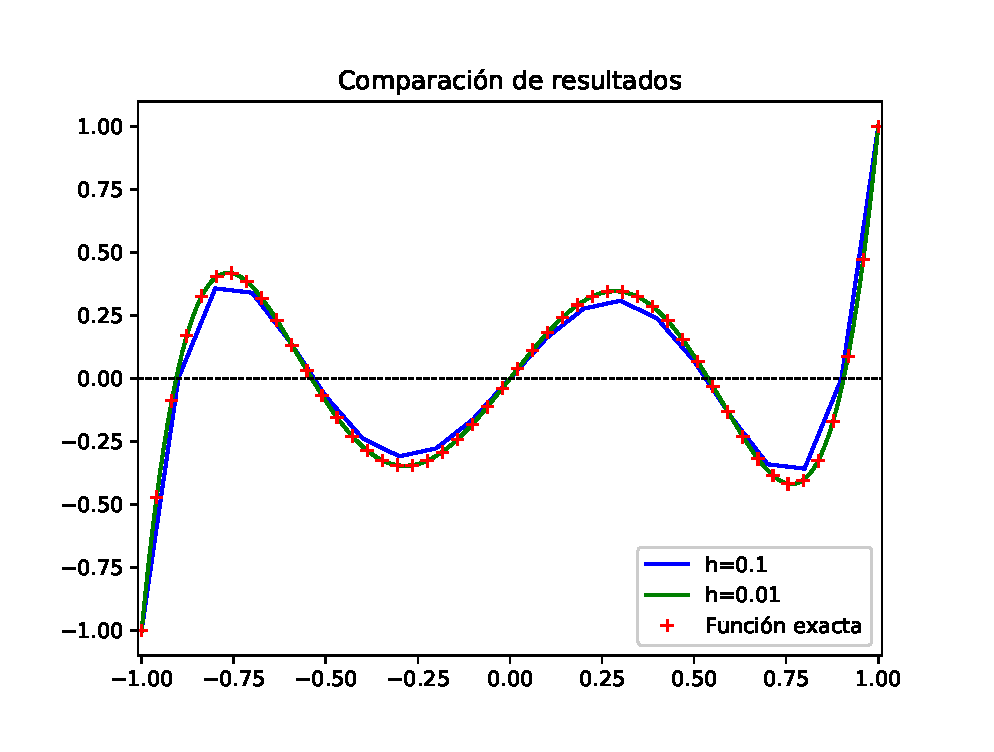
\includegraphics[scale=0.6]{Imagenes/ejercicio_Legendre_01.eps}
\end{figure}
\end{frame}
\begin{frame}
\frametitle{¿Cómo graficamos los resultados?}
Para graficar los archivos de texto que obtuvimos (se guardó uno con el valor de $h=0.1$ y el otro con $h=0.01$), podemos recuperar los valores a listas y ocupar las rutinas conocidas previamente.
\end{frame}
\begin{frame}
\frametitle{La función \texttt{genfromtxt}}
Para recuperar el conjunto de datos de un archivo de una manera mucho más rápida y sencilla, usamos la función \funcionazul{genfromtxt}:
\\
\bigskip
Que carga el conjunto de datos contenido en un archivo de texto plano.
\end{frame}
\begin{frame}[fragile]
\frametitle{Usando la función \texttt{genfromtxt}}
Debemos de asignar en una variable el contenido de datos que guardamos en cada archivo, mediante \funcionazul{genfromtxt}:
\begin{lstlisting}[caption=Función \texttt{genfromtxt}, style=FormattedNumber, basicstyle=\linespread{1.1}\ttfamily=\small, columns=fullflexible]

mat_0_ = np.genfromtxt("bilocalh0_\textunderscore_1.txt")

mat_1_ = np.genfromtxt("bilocalh0_\textunderscore_01.txt")
\end{lstlisting}
\end{frame}
\begin{frame}[fragile]
\frametitle{Comparando con la función exacta}
El problema pide que comparemos la solución obtenida por el procedimiento de diferencias finitas contra el valor de la función exacta, por ello, nos apoyamos con la función especial \funcionazul{scipy.special.legendre}:
\end{frame}
\begin{frame}[fragile]
\begin{lstlisting}[caption=Evaluando la función de Legendre, style=FormattedNumber, basicstyle=\linespread{1.1}\ttfamily=\small, columns=fullflexible]   
from scipy.special import legendre as splegendre

xj_5_ = np.linspace(-1., 1.)

j_5_ = np.polyval(splegendre(5), xj_5_)
\end{lstlisting}
\end{frame}
\begin{frame}[fragile]
\frametitle{Graficando las funciones}
Por último nos resta incluir la rutina de graficación que ya manejamos con facilidad y así obtenemos la gráfica con las tres curvas:
\end{frame}
\begin{frame}[plain, allowframebreaks, fragile]
\frametitle{Graficando las funciones}
\begin{lstlisting}[caption=Rutina de graficación, style=FormattedNumber, basicstyle=\linespread{1.1}\ttfamily=\small, columns=fullflexible]
import matplotlib.pyplot as plt

plt.plot(mat_0_[:,_0_], mat_0_[:,_1_], 'b', label = "h=0.1")
plt.plot(mat_1_[:,_0_], mat_1_[:,_1_], 'g', label = "h=0.01")
plt.plot(xj_5_, j_5_, 'r+', label='Funcion exacta')
plt.axhline(y=0, ls='dashed', lw=0.7, color='k')
plt.title('Comparacion de resultados')
plt.xlim([-1.01, 1.01])
plt.legend(loc='lower right')
plt.show()
\end{lstlisting}
\end{frame}
\begin{frame}
\frametitle{Comparando los resultados obtenidos}
\begin{figure}
   \centering
   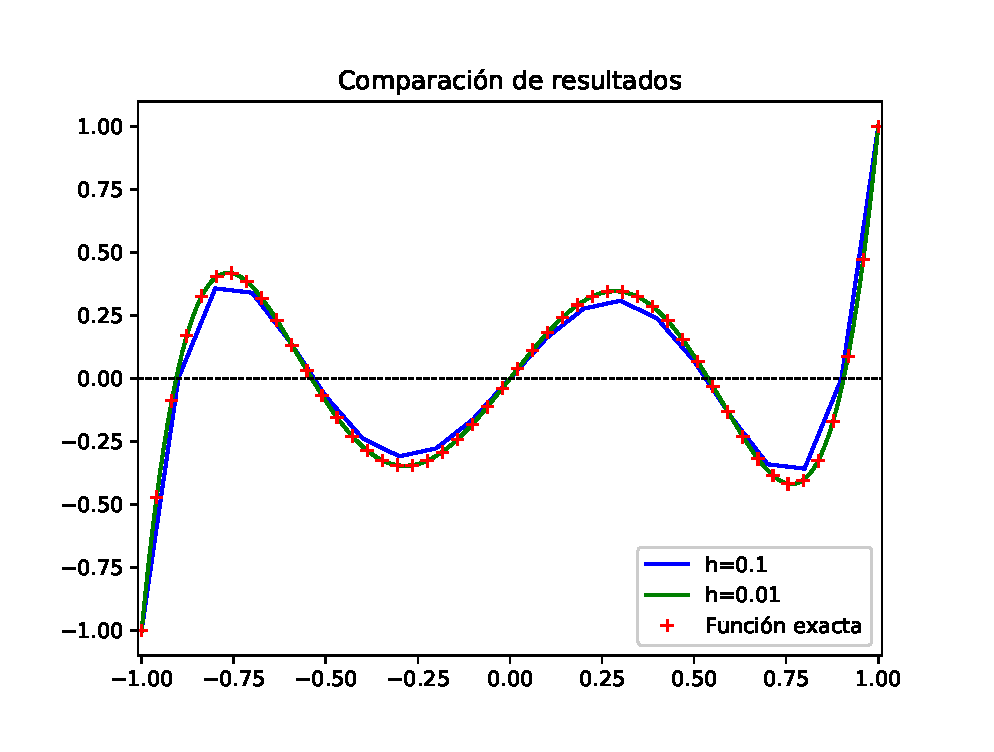
\includegraphics[scale=0.6]{Imagenes/ejercicio_Legendre_01.eps}
\end{figure}
\end{frame}
\begin{frame}
\frametitle{Ejercicios a cuenta de examen}
Los siguientes ejercicios son a cuenta del examen parcial:
\setbeamercolor{item projected}{bg=blue!70!black,fg=white}
\setbeamertemplate{enumerate items}[circle]
\begin{enumerate}[<+->]
\item Usando el método de disparo resuelve para el polinomio de Legendre de orden $5$, es decir $P_{5}(x)$ y compara la solución con el método de diferencias finitas que se menciona en el ejercicio anterior.
\seti
\end{enumerate}
\end{frame}
\begin{frame}
\frametitle{Ejercicios a cuenta de examen}
\setbeamercolor{item projected}{bg=blue!70!black,fg=white}
\setbeamertemplate{enumerate items}[circle]
\begin{enumerate}[<+->]
\conti
\item Usando el método de diferencias finitas con CDF, resuelve para los polinomios de Chebychev de primera clase
\[ \begin{split} \dfrac{d^{2} T_{n}}{d x^{2}} = \dfrac{1}{1 - x{2}} \left[ x \: \dfrac{d T_{n}}{d x} - n^{2} \: T_{n} \right] \\
\\
T_{n}(-1) = (-1)^{n} \hspace{0.5cm} T_{n}(1) = 1
\end{split} \]
Usando un tamaño de paso de $h = 10^{-4}$. Calcula y gráfica los polinomios $T_{n}$ de primera clase de orden $n = 1, 2, \ldots, 5$.
\seti
\end{enumerate}
\end{frame}
\begin{frame}
\frametitle{Ejercicios a cuenta de examen}
\setbeamercolor{item projected}{bg=blue!70!black,fg=white}
\setbeamertemplate{enumerate items}[circle]
\begin{enumerate}[<+->]
\conti
\item Un cilindro grueso transporta un fluido con una temperatura de $\SI{0}{\celsius}$. Al mismo tiempo, el cilindro se sumerge en un baño que se mantiene a $\SI{200}{\celsius}$.
\end{enumerate}
\begin{figure}
	\centering
	\includestandalone[scale=0.8]{Figuras/fig_edo_cdf_cilindro_01}
\end{figure}
\end{frame}
\begin{frame}
\frametitle{EDO y CDF}
La ecuación diferencial y las CDF que determinan la conducción de calor en estado estacionario en el cilindro son
\[ \dfrac{d^{2} T}{d r^{2}} = -\dfrac{1}{r} \dfrac{d T}{d r} \hspace{0.5cm} T_{\vert r = a/2} = \SI{0}{\celsius} \hspace{0.5cm} T_{\vert r = a} = \SI{200}{\celsius} \]
donde $T$ es la temperatura.
\end{frame}
\begin{frame}
\frametitle{Problema a resolver}
Determina el perfil de temperatura a través del cilindro usando el método de diferencias finitas, compara tu resultado con la solución analítica:
\[ T =  200 \left( 1 - \dfrac{\ln r/a}{\ln 0.5} \right) \]
\end{frame}
\end{document}